Uma extensão para a aplicação \textit{my5G-RANTester} foi desenvolvida utilizando-se como base o trabalho de \citeonline{Dominato2021}.
Essa prova de conceito teve o intuito de avaliar o comportamento das diferentes implementações de código aberto de núcleo 5G para execução dos procedimentos em escala.
O trabalho de \citeonline{Dominato2021} implementa um testador que tem como objetivo simular e realizar testes sobre os planos de controle e de dados de UEs e de estações de rádio base da rede 5G.
O testador foi projetado para realizar testes de conformidade e robustez sobre diferentes implementações de código aberto de núcleos de redes 5G.
Todavia, o testador suporta a expansão para outras cargas de trabalhos, permitindo o desenvolvimento de outros tipos de testes, como os testes de desempenho que estão sendo abordados nesta presente pesquisa.

A arquitetura em alto nível da aplicação desenvolvida por \citeonline{Dominato2021} pode ser vista na Figura \ref{fig:tester_arch}.
A prova de conceito, desenvolvida na linguagem de programação \textit{Go}\footnote{Linguagem criada pela Google em 2009 (https://go.dev)}, implementa as camadas de Simulação, do Controlador e da Interface de usuário.
A camada de Simulação imita o comportamento de uma ou mais gNB e de um ou mais UEs.
\citeonline{Dominato2021} simulam em seu estudo múltiplas conexões gNB e UEs em sequência. Na presente pesquisa, a simulação foi realizada com múltiplas conexões gNB e UEs simultâneas com o intuito de validar a performance de cada implementação de núcleo da rede.

A camada do Controlador é a principal camada no funcionamento do testador. Essa camada recebe os comandos do usuário através de uma interface que define qual teste será executado, controla a camada acima e faz a coleta das métricas do experimento.
Os planos de testes representam os testes em si que foram escolhidos para serem executados. O Executor recebe as informações do teste, configura as gNB e os UEs e envia as métricas para o Coletor de métricas, que irá armazená-las para futuros usos.
O presente trabalho estende o módulo do plano de testes, adicionando a possibilidade de executar testes de conectividade de UEs em paralelo, permitindo medir o comportamento do núcleo da rede operando sobre maior carga de trabalho.

Por fim, a camada da Interface de usuário permite a execução e o monitoramento dos testes, além de exportar as métricas armazenadas na camada acima. É com essa camada que o usuário do testador pode interagir através de parâmetros enviados por uma linha de comandos a ser executada no ambiente de testes.


\begin{figure}[!ht]
    \centering
    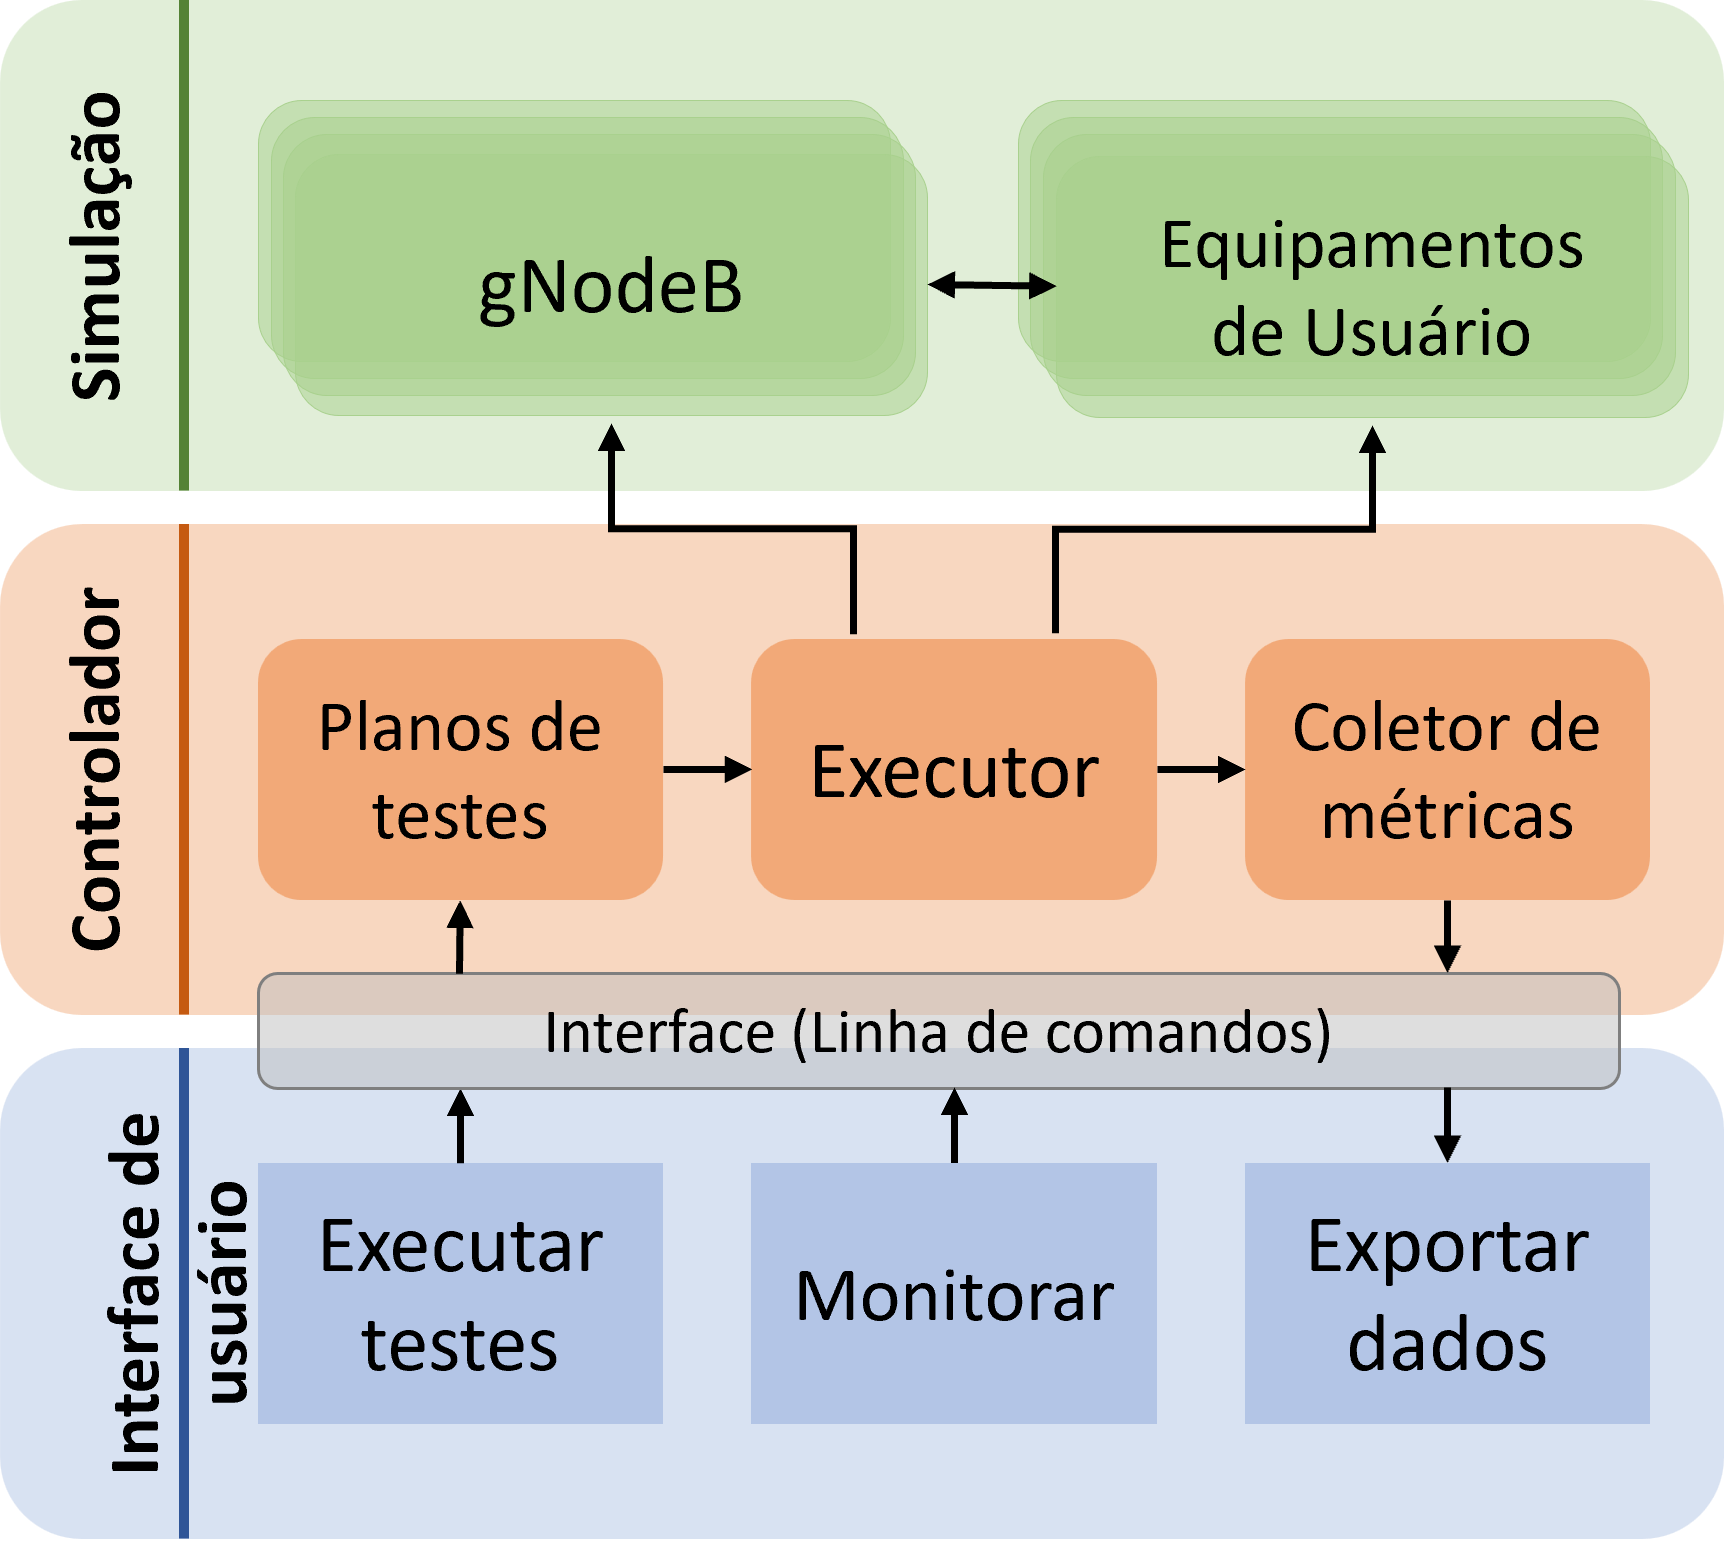
\includegraphics[width=0.6\textwidth]{TG2/Chapters/Soluction/Figures/Arquitetura-Componentes.png}
    \caption{Arquitetura do testador}
    \label{fig:tester_arch}
\end{figure}


Para desenvolver este trabalho, além do módulo implementado internamente no testador, também foi necessário desenvolver algumas ferramentas para a automação da criação e configuração do ambiente de testes e da execução dos experimentos. Essas ferramentas orquestram as múltiplas execuções dos experimentos e coletam os dados gerados para análise futura. A seguir, são apresentadas as ferramentas desenvolvidas no decorrer deste trabalho.

\subsection{Módulo de teste}

Para a execução de testes de desempenho, foi desenvolvido um módulo para o testador que permite a execução de múltiplas conexões de UEs simultâneas.
Esse módulo foi implementado suportando parâmetros de configuração para facilitar variações entre os testes. 
Desta forma, é possível definir o número de UEs a serem conectados, o atraso em milissegundos (ms) entre uma conexão e outra e o atraso em segundos (s) para começar a execução do experimento.

No começo da execução, esse módulo simula uma gNB e inicia a conexão com o núcleo da rede. Após a conexão ser bem sucedida, é aguardado o tempo para iniciar a execução do experimento.
Ao iniciar o experimento, o módulo inicia um fluxo de trabalho em paralelo para criar uma nova instância de UE e realizar a conexão com o núcleo da rede.
Após iniciar o fluxo de trabalho em paralelo, o módulo aguarda o atraso entre conexões definido pelo usuário antes de iniciar o próximo fluxo, até que a quantidade de dispositivos definida seja atingida.

Durante a etapa de desenvolvimento do módulo, foi descoberta uma limitação na implementação do testador, que não consegue gerenciar mais que 255 UEs conectados simultaneamente.
Analisando o código, observa-se que a correção da limitação necessitaria de tempo e recursos não previstos na presente pesquisa.
Foi feito um contato com os desenvolvedores do testador sobre essa limitação, mas a solução para o problema não foi implementada até o presente momento.
Sendo assim, foi decidido criar múltiplas instâncias do testador, cada uma simulando uma gNB diferente, todas se conectando de forma simultânea na mesma instância do núcleo, cada uma simulando uma quantidade predefinida de UEs.
Desse modo, foi possível testar o comportamento de um núcleo de rede 5G com múltiplos UEs e gNB.

\subsection{Módulo de coleta de dados do testador}

O módulo de coleta de dados consiste em um fluxo de execução em paralelo que registra o tempo, em nanossegundos (ns), que cada UE demorou para trocar entre cada estado da conexão com o núcleo da rede 5G.
As informações de tempo para cada estado de cada UE são escritas na saída de texto padrão do contêiner utilizado pela instância do testador.
Esse módulo foi implementado nesta presente pesquisa, visto que o testador não possuía suporte para a coleta dessa métrica até o presente momento.

Ao final da execução, uma aplicação foi desenvolvida para realizar o processamento das informações geradas através das diversas instâncias do testador, fazendo um pré processamento dos dados, ordenando eles com base no horário da inicialização do UE (em ns a partir do \textit{epoch time}\footnote{\textit{Epoch time} é uma unidade de medida de tempo contada a partir da data 1 de janeiro de 1970 às 00:00:00 UTC.}) e gerando um arquivo de texto separado por vírgulas, permitindo a fácil importação dos resultados através de programas de análise de dados.
Inicialmente, essa aplicação foi desenvolvida para coletar e processar os registros de uma única instância do testador, ordenando em ordem crescente pelo identificador do UE os dados no arquivo de saída.
Entretanto, foi necessário modificar essa aplicação para suportar múltiplas instâncias de testadores executando em paralelo e reordenar os dados do arquivo de saída, visto que a ordem de conexão dos dispositivos deixou de ser realizada em ordem crescente do identificador.

A aplicação consiste em um \textit{script} escrito na linguagem \textit{JavaScript}\footnote{https://developer.mozilla.org/pt-BR/docs/Web/JavaScript} que é executado dentro de um contêiner \textit{Docker}, evitando a instalação de um interpretador de \textit{JavaScript} diretamente na máquina que está executando os experimentos.

\subsection{Módulo de coleta de dados do núcleo}

O desenvolvimento deste módulo teve a contribuição dos bolsistas de iniciação científica do projeto PORVIR-5G.
Esse módulo consiste na implementação de um fluxo sobre uma instância da aplicação \textit{Node-RED}\footnote{https://nodered.org/}.
Um fluxo foi desenvolvido para listar todos os contêineres em execução na máquina e realizar a coleta das métricas do \textit{Docker} e armazená-las em uma instância do banco de dados \textit{InfluxDB}\footnote{https://www.influxdata.com/}. Esse fluxo foi definido para ser executado automaticamente após a inicialização do contêiner do \textit{Node-RED}, permitindo a coleta de dados de uso de disco, rede, processador, memória, entre outras, de forma automatizada pelo orquestrador do experimento.

\subsection{Orquestrador}
\label{sub:arch-orchestrator}

Com o objetivo de realizar todas as execuções dos experimentos de forma mais semelhante possível, foi desenvolvido um orquestrador que gerencia toda a execução do experimento.
O orquestrador consiste em uma série de roteiros de execução, desenvolvidos em sua maioria sobre as linguagens \textit{Bash Script} e \textit{JavaScript}.
A Figura \ref{fig:flux_orq} representa um fluxograma do algoritmo de execução do orquestrador.
O orquestrador é executado através de uma interface de usuário por linha de comandos, suportando diversos comandos para definir os parâmetros de execução do experimento, permitindo ao usuário automatizar a execução de experimentos de forma simplificada.

Os parâmetros suportados são a quantidade total de UEs a serem conectados no núcleo da rede, a quantidade de testadores que serão executados em paralelo, o tempo em ms para ser aguardado entre cada conexão de UE, o tempo em s para aguardar a inicialização, qual núcleo da rede 5G deve ser utilizado para executar o experimento e qual experimento será executado.
Além dos parâmetros de execução do experimento, o orquestrador também permite o usuário interromper a última execução e limpar o ambiente de testes, removendo todos os contêineres e dados gerados pelo experimento, além de permitir executar o orquestrador em modo de depuração, exibindo para o usuário todos os registros de execução.

Ao iniciar a execução do orquestrador, será feita uma análise sobre o sistema operacional, verificando se a versão necessária do \textit{Kernel} do sistema está instalada.
Após realizar esta validação, o orquestrador irá verificar se todas as dependências estão corretamente instaladas e configuradas. Caso contrário, o orquestrador fará as devidas modificações automaticamente.
Uma vez que o sistema está pronto, é iniciada a execução do experimento desejado.
Primeiramente, o código-fonte do núcleo da rede 5G escolhido será baixado, compilado e seus arquivos binários serão armazenados em uma imagem de contêiner \textit{Docker}, que será iniciada na sequência.
Após a inicialização do núcleo, a base de dados desse núcleo é preenchida com as informações necessárias para a conexão dos UEs de acordo com as configurações do experimento.
Concluindo-se essa etapa, é iniciado o módulo de coleta de dados do núcleo, descrito anteriormente.
Por fim, inicia-se o contêiner do testador com os parâmetros definidos pelo usuário.

O orquestrador foi desenvolvido para suportar diferentes implementações de núcleos da rede 5G. Para isso, foi desenvolvida uma interface genérica para a inicialização do núcleo. Assim, para adicionar o suporte a um novo núcleo, basta implementar essa interface para o núcleo desejado e adicioná-la ao orquestrador.
Para a realização deste trabalho, foi desenvolvido o suporte para as implementações de núcleo 5G \textit{free5GC}, \textit{Open5GS} e OAI.
Todos os códigos fontes utilizados no desenvolvimento da presente pesquisa encontram-se no repositório do projeto PORVIR-5G\footnote{https://github.com/PORVIR-5G-Project} disponível através da plataforma \textit{GitHub}.

\begin{figure}[!ht]
    \centering
    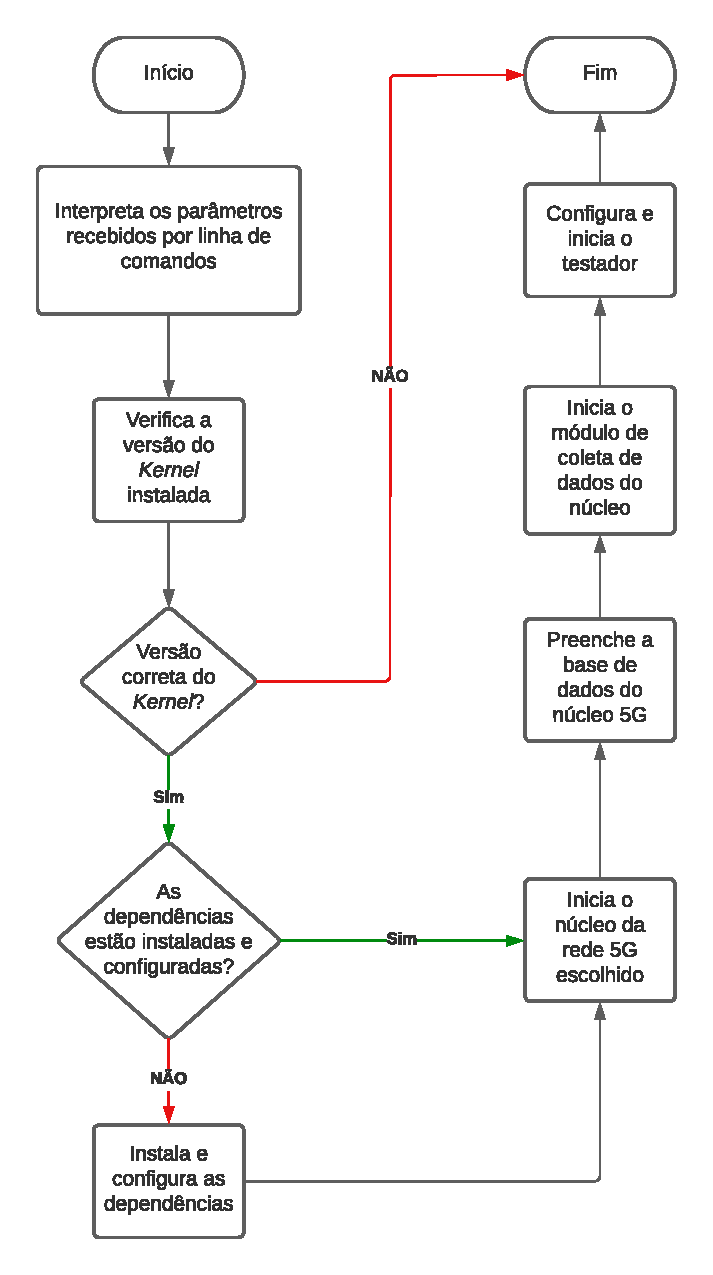
\includegraphics[width=0.65\textwidth]{TG2/Chapters/Soluction/Figures/Fluxograma-Orquestrador.pdf}
    \caption{Fluxograma de execução do orquestrador}
    \label{fig:flux_orq}
\end{figure}
